\subsection{最优传输问题}\label{sec:1.1}

Monge 在其 1781 年的论文\cite{ref231}中提出了如下问题：怎样把一堆给定的沙子搬运过去，填满一个给定的沟渠，并使搬运沙子的成本最小？这个问题可以用概率分布建模. 首先注意，要使这项任务能够完成，沙堆与沟渠必须具有相同的体积. 不失一般性，将这个体积归一化为 $1$. 由此，我们需要考虑 $\mathbb R^d$ 上的两个概率测度 $\mu$ 和 $\nu$. 借助两个随机变量 $X\sim\mu$、$Y\sim\nu$ 来思考通常更方便. 它们就是这个约束优化问题的输入.

\subsubsection{Monge 问题与 Kantorovich 问题}\label{sec:1.1.1}

回到搬沙子的类比，搬运沙堆意味着寻找一个称为\emph{传输映射}（transport map）的可测函数 $T:\mathbb R^d\to\mathbb R^d$，它规定位于 $x\in\mathbb R^d$ 的沙子应搬到 $T(x)\in\mathbb R^d$. 要让传输映射真正完成任务，即填满沟渠，就必须保证只要 $X\sim\mu$，便有 $T(X)\sim\nu$. 此时称 $T$ 将 $\mu$ \emph{推前}至 $\nu$，或者称 $\nu$ 是 $\mu$ 经由 $T$ 得到的\emph{推前测度}（pushforward measure），记为 $T_\#\mu=\nu$. 这就是我们的约束.

现在来看目标函数. 回顾 Monge 的问题，我们要使搬运沙子的成本最小. 成本可以用许多方式衡量，例如体力消耗或燃料消耗等. 为简化叙述，这里仅用沙子移动的欧氏距离来衡量. 位于 $x$ 的沙子移动的距离为 $\lVert T(x)-x\rVert$. 因而，平均移动距离为
$$
\int\lVert T(x)-x\rVert\,\mu(dx).
$$
因此，最优传输问题（optimal transport problem）的 Monge 表述\index{Monge problem@Monge问题（Monge problem）|hyperpage}，是在 $T$ 将 $\mu$ 推前至 $\nu$ 的约束下，使上述目标最小化：
$$
\inf_{T:T_\#\mu=\nu}\int\lVert T(x)-x\rVert\,\mu(dx).
$$
注意，传输成本还有许多其他选择. 最一般地，通常考虑一般成本 $c(X,T(X))$，其中 $c(x,y)$ 衡量把 $x\in\mathbb R^d$ 搬到 $y\in\mathbb R^d$ 的成本. 在这一一般框架下，甚至可以允许 $X$ 和 $Y$ 定义在两个不同的空间上，而不必都是 $\mathbb R^d$. 本讲义主要关注 $c(x,y)=\lVert x-T(x)\rVert$ 或 $c(x,y)=\lVert x-T(x)\rVert^2$ 的情形，它们导出 Wasserstein 距离（Wasserstein distance）. 空间 $\mathbb R^d$ 也可以换成更复杂的空间，例如黎曼流形，但这通常超出了本讲义的范围（\autoref{sec:5.6}除外）.

虽然 Monge 问题很容易表述，但仍有几个问题需要回答：
\begin{itemize}
\item 这样的有效传输映射是否总是存在？反过来说，约束集合是否可能为空？
\item 如果存在极小化解，它是否唯一？如何刻画它？注意，我们的约束不是凸的，因此这个问题相当难以回答.
\end{itemize}
一个简单的例子便能回答第一个问题. 取 $d=1$，设 $\mu=\delta_0$ 是位于 $0$ 的点质量，而 $\nu=\frac12\delta_{-1}+\frac12\delta_1$ 是两个点质量的混合. 无论怎样选择传输映射 $T$，推前测度 $T_\#\mu$ 都是位于 $T(0)$ 的点质量 $\delta_{T(0)}$，因此根本无法完成传输，至少确定性映射做不到.

直观地，我们希望有
$$
T(0)=\begin{cases}
-1,&\text{以概率 }\frac12,\\
1,&\text{以概率 }\frac12,
\end{cases}
\qquad\text{且}\qquad
T(x)=x,\quad\forall x\ne0.
$$
这样的 $T$ 不是函数，而是一个 Markov 核（Markov kernel）：它为每个点 $x\in\mathbb R$ 指定一个概率分布.

第二个问题在此后近两个世纪中一直没有令人满意的答案，直到苏联数学家 Leonid Kantorovich 在一篇具有开创性的两页论文\cite{ref173}中引入了该问题的一个松弛形式，恰好允许使用上例所讨论的 Markov 核. 等价地，这种表述涉及的是耦合，而不是映射.

设 $\mu,\nu$ 是 $\mathbb R^d$ 上的两个概率测度，$\gamma$ 是这两个分布的一个\emph{耦合}（coupling），即 $\mathbb R^d\times\mathbb R^d$ 上的一个联合分布，其第一边缘分布为 $\mu$，第二边缘分布为 $\nu$：对于任意 Borel 集 $A\in\mathbb R^d$，有
$$
\gamma(A\times\mathbb R^d)=\mu(A)
\qquad\text{且}\qquad
\gamma(\mathbb R^d\times A)=\nu(A).
$$
之所以使用“耦合”一词，是因为原本 $X\sim\mu$ 与 $Y\sim\nu$ 是互不相关的两个随机变量，而耦合通过描述它们的概率依赖关系，使它们处在同一个概率空间上. 本讲义以下始终用 $\Gamma_{\mu,\nu}$ 表示 $\mu$ 和 $\nu$ 的所有耦合组成的集合.

设 $c:\mathbb R^d\times\mathbb R^d\to[0,\infty)$ 是可测成本函数. 最优传输问题的一般 Kantorovich 表述就是下面的优化问题：
\begin{equation}\tag{KOT}\label{eq:KOT}\index{Kantorovich problem@Kantorovich问题（Kantorovich problem）|hyperpage}
\inf_{\gamma\in\Gamma_{\mu,\nu}}\int c(x,y)\,\gamma(dx,dy).
\end{equation}

\subsubsection{耦合}\label{sec:1.1.2}

为了更好地理解 Kantorovich 问题，考察集合 $\Gamma_{\mu,\nu}$ 很有帮助.

也许最简单的耦合是\emph{独立耦合}（independent coupling）$\gamma=\mu\otimes\nu$，这里仅假设 $X\sim\mu$ 与 $Y\sim\nu$ 相互独立：对于任意 Borel 集 $A,B\subseteq\mathbb R^d$，
$$
\gamma(A\times B)=\mu(A)\cdot\nu(B).
$$
下一个命题汇集了关于 $\Gamma_{\mu,\nu}$ 的一些初步事实.

\begin{proposition}\label{prop:1.1}
设 $\mu,\nu$ 是 $\mathbb R^d$ 上的两个概率测度. 两者的耦合集合 $\Gamma_{\mu,\nu}$ 非空、凸，并且在弱收敛拓扑下是紧的.
\end{proposition}
\begin{proof}
由于独立耦合总是存在，所以 $\Gamma_{\mu,\nu}\ne\varnothing$.

为证明 $\Gamma_{\mu,\nu}$ 是凸的，考虑两个耦合 $\gamma_0,\gamma_1\in\Gamma_{\mu,\nu}$，对任意 $\lambda\in(0,1)$ 定义混合 $\gamma_\lambda=(1-\lambda)\gamma_0+\lambda\gamma_1$. 注意，对于任意 Borel 集 $A\in\mathbb R^d$，
$$
\begin{aligned}
\gamma_\lambda(A\times\mathbb R^d)
&=(1-\lambda)\gamma_0(A\times\mathbb R^d)+\lambda\gamma_1(A\times\mathbb R^d)\\
&=(1-\lambda)\mu(A)+\lambda\mu(A)=\mu(A).
\end{aligned}
$$
因此 $\gamma_\lambda$ 的第一边缘分布为 $\mu$，同理，其第二边缘分布为 $\nu$. 所以任意 $\lambda\in(0,1)$ 都有 $\gamma_\lambda\in\Gamma_{\mu,\nu}$，从而 $\Gamma_{\mu,\nu}$ 是凸的.

为完成这个命题的证明，我们证明 $\Gamma_{\mu,\nu}$ 是紧的. 根据 Prokhorov 定理（\autoref{thm:B.3}），只需证明 $\Gamma_{\mu,\nu}$ 是闭的且（一致）紧的测度族. 为此，回顾 Prokhorov 定理可知，常值序列 $(\mu)_n$、$(\nu)_n$ 都是紧的，因而对任意 $\varepsilon>0$，存在紧集 $K\subset\mathbb R^d$ 使 $\mu(K^c)+\nu(K^c)<\varepsilon$. 于是 $K\times K$ 也是紧集，且对任意 $\gamma\in\Gamma_{\mu,\nu}$，
$$
\begin{aligned}
\gamma\bigl((K\times K)^c\bigr)
&\le\gamma(\mathbb R^d\times K^c)+\gamma(K^c\times\mathbb R^d)\\
&=\mu(K^c)+\nu(K^c)<\varepsilon.
\end{aligned}
$$
因此 $\Gamma_{\mu,\nu}$ 是紧的测度族. 此外，$\gamma\in\Gamma_{\mu,\nu}$ 等价于：对所有有界连续函数 $f:\mathbb R^d\to\mathbb R$，
$$
\int f(x)\,\gamma(dx,dy)=\int f\,d\mu
\qquad\text{且}\qquad
\int f(y)\,\gamma(dx,dy)=\int f\,d\nu.
$$
由弱收敛的定义（\autoref{thm:B.4}）可知 $\Gamma_{\mu,\nu}$ 是闭的. 因此，Prokhorov 定理表明 $\Gamma_{\mu,\nu}$ 是紧的.
\end{proof}

耦合 $\gamma\in\Gamma_{\mu,\nu}$ 刻画两个随机变量 $X\sim\mu$ 与 $Y\sim\nu$ 之间的依赖关系. 如上所述，一种选择是假设 $X$ 与 $Y$ 独立，由此得到独立耦合. 在\autoref{fig:1.1}（左）中，我们绘出了两个高斯混合分布之间的独立耦合. 作为独立耦合的另一个极端，举例来说，设 $X\sim\mathcal N(0,1)$、$Y\sim\chi_1^2$，注意 $Y$ 与 $X^2$ 同分布. 因此可以采用满足 $Y=X^2$ 的\emph{确定性耦合}（deterministic coupling）：
$$
\gamma(dx,dy)=\mu(dx)\,\delta_{x^2}(dy).
$$
我们在\autoref{fig:1.1}（右）中绘出了这个耦合；注意它是退化的.

\begin{figure}[htbp]
\centering
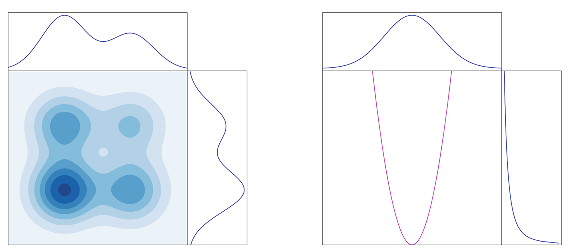
\includegraphics[width=\linewidth]{assets/chapter1/fig1-1.pdf}
\caption{（左）两个高斯分布的混合分布之独立耦合.（右）$X\sim\mathcal N(0,1)$ 与 $Y\sim\chi_1^2$ 的确定性耦合.}\label{fig:1.1}
\end{figure}

\begin{figure}[htbp]
\centering
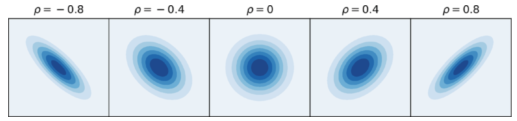
\includegraphics[width=\linewidth]{assets/chapter1/fig1-2.pdf}
\caption{$\rho$ 取五个不同值时，\eqref{eq:1.1} 所示的二元高斯耦合.}\label{fig:1.2}
\end{figure}

继续考察耦合，假设 $X\sim\mathcal N(0,1)$、$Y\sim\mathcal N(0,1)$，则可以采用任意满足下式的耦合：
\begin{equation}\label{eq:1.1}
\begin{pmatrix}X\\Y\end{pmatrix}
\sim\mathcal N\!\left(\begin{pmatrix}0\\0\end{pmatrix},
\begin{pmatrix}1&\rho\\\rho&1\end{pmatrix}\right),
\end{equation}
其中 $\rho\in[-1,1]$ 是 $X$ 与 $Y$ 的相关系数，见\autoref{fig:1.2}.

本章后面的 Brenier 定理表明，在温和的正则条件下，二次成本 Kantorovich 问题的解由一个确定性耦合达到. 正如下文将讨论的，当 $\mu$ 和 $\nu$ 是离散测度时，可以通过考察集合 $\Gamma_{\mu,\nu}$ 的几何来理解这一事实.

\subsubsection{离散最优传输}\label{sec:1.1.3}

$\mu$ 和 $\nu$ 为两个离散分布的情形，在实践中尤其重要. 例如，$\mu,\nu$ 可以是点云上的经验测度. 考虑
$$
\mu=\sum_{i=1}^m p_i\delta_{x_i},
\qquad\text{且}\qquad
\nu=\sum_{j=1}^n q_j\delta_{y_j}.
$$
此时，$X\sim\mu$ 与 $Y\sim\nu$ 的耦合 $\gamma$ 可由非负矩阵 $P\in\mathbb R^{m\times n}$ 刻画，其中 $P_{i,j}=\gamma(X=x_i,Y=y_j)$. $\gamma\in\Gamma_{\mu,\nu}$ 的边缘约束直接转化为
$$
\forall i\in[m],\quad\sum_{j\in[n]}P_{i,j}=p_i,
\qquad\text{且}\qquad
\forall j\in[n],\quad\sum_{i\in[m]}P_{i,j}=q_j.
$$
分别用 $\mathbf1_m$、$\mathbf1_n$ 表示长度为 $m$、$n$ 的全一向量，这些约束就可简洁地表示为 $P\mathbf1_n=p$、$P^{\mathsf T}\mathbf1_m=q$，其中 $p=(p_1,\ldots,p_n)^{\mathsf T}$、$q=(q_1,\ldots,q_m)^{\mathsf T}$.

与耦合类似，成本 $c$ 也可以由一个 $m\times n$ 矩阵 $C$ 表示，其中 $C_{i,j}=c(x_i,y_j)$，$i\in[m]$、$j\in[n]$. 因此 Kantorovich 最优传输问题 \eqref{eq:KOT} 等价于
$$
\min_{P\in\mathbb R_+^{m\times n}}\sum_{i,j\in[n]}C_{i,j}P_{i,j}
\qquad\text{满足}\qquad
P\mathbf1_n=p,\quad P^{\mathsf T}\mathbf1_m=q,
$$
也可以更简洁地写为
$$
\min_{P\in\mathbb R_+^{m\times n}}\langle C,P\rangle
\qquad\text{满足}\qquad
P\mathbf1_n=p,\quad P^{\mathsf T}\mathbf1_m=q,
$$
其中 $\langle C,P\rangle=\operatorname{tr}(C^{\mathsf T}P)$ 是实 $m\times n$ 矩阵空间上的 Frobenius 内积.

特别地，当 $m=n$，并且所有权重 $p_i$、$q_j$ 均为 $1/n$ 时，有效耦合矩阵 $P$ 的集合就是双随机矩阵集合的一个倍数，后者也称为 Birkhoff\index{Birkhoff polytope@Birkhoff多面体（Birkhoff polytope）|hyperpage} 多面体（Birkhoff polytope）：
\begin{equation}\label{eq:1.2}
\operatorname{Birk}:=\{\gamma\in\mathbb R_+^{n\times n}:\gamma\mathbf1_n=\mathbf1_n,\ \mathbf1_n^{\mathsf T}\gamma=\mathbf1_n^{\mathsf T}\}.
\end{equation}
此时，\eqref{eq:KOT} 化为
\begin{equation}\label{eq:1.3}
\min_{P\in n^{-1}\operatorname{Birk}}\langle C,P\rangle.
\end{equation}
Birkhoff 多面体的极点是置换矩阵：它们是二元矩阵 $\pi\in\{0,1\}^{n\times n}$，每行每列恰有一个非零元素. 特别地，根据凸几何的一般原理，形如 \eqref{eq:1.3} 的任意线性规划都可以取一个形如 $n^{-1}\pi$ 的矩阵作为解. 这种形式的传输方案由一个确定性映射（即置换）诱导，因此此时 Monge 问题有解. 正如后续各节将展示的，更一般地，$\Gamma_{\mu,\nu}$ 的极点在最优传输问题的几何中扮演着特殊角色.
